\begin{figure}[h]
    \centering
    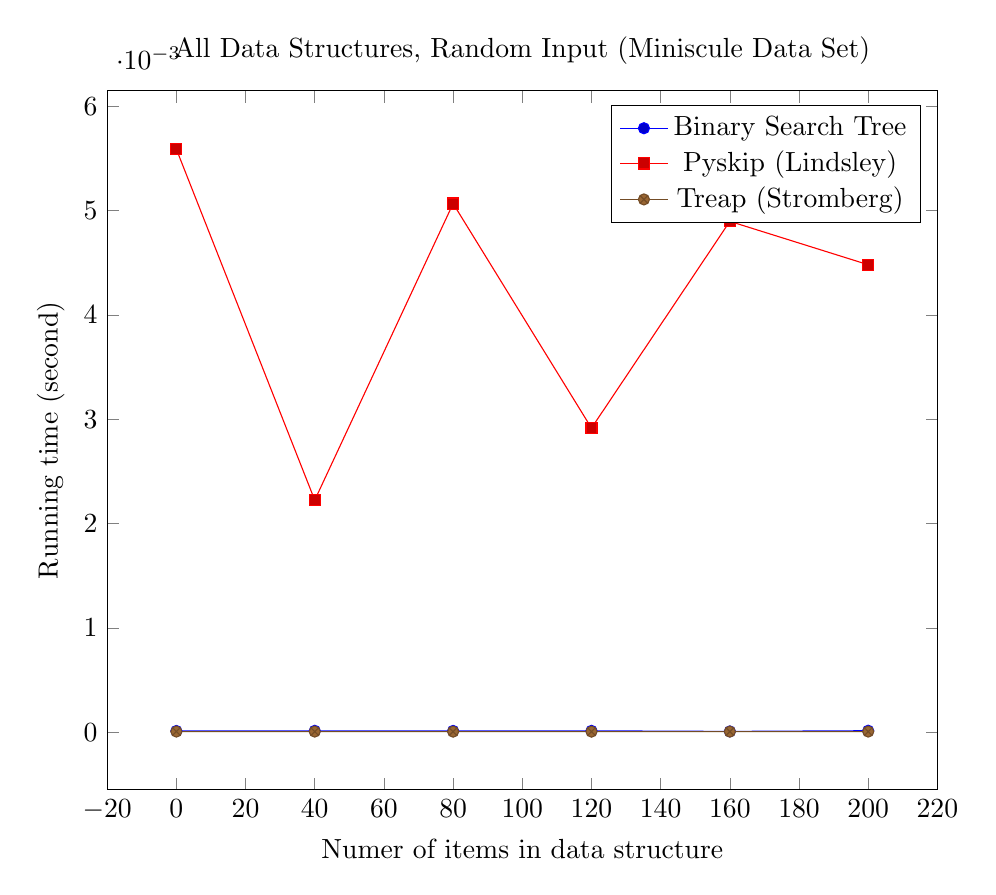
\begin{tikzpicture}
        \begin{axis}[
            xlabel={Numer of items in data structure},
            ylabel={Running time (second)},
            title={All Data Structures, Random Input (Miniscule Data Set)},
            width=\textwidth
        ]
		\addplot coordinates {
			(0, 1.1023017325118012e-05)
			(40, 1.255901154253447e-05)
			(80, 1.1685603065969552e-05)
			(120, 1.2318071273131892e-05)
			(160, 6.89691521160718e-06)
			(200, 1.3432420019121594e-05)
		};
		\addplot coordinates {
			(0, 0.005590266013116185)
			(40, 0.002224571389848884)
			(80, 0.005068871270131692)
			(120, 0.00291579890522764)
			(160, 0.004898165089260842)
			(200, 0.004482211831673122)
		};
		\addplot coordinates {
			(0, 5.511508662525699e-06)
			(40, 5.360920994190721e-06)
			(80, 4.607982652338194e-06)
			(120, 4.698335253294772e-06)
			(160, 4.969393056386551e-06)
			(200, 5.330803460479317e-06)
		};
        \legend{Binary Search Tree, Pyskip (Lindsley), Treap (Stromberg)}
        \end{axis}
    \end{tikzpicture}
    \caption{Average of 10 operations, benchmarked every 40, starting at 0.}
\end{figure}